% !TeX spellcheck = en_GB
% !TeX program = pdflatex
%
% LetzCV-sleek 1.0 LaTeX template
% Author: Andreï V. Kostyrka, University of Luxembourg
%
% This template fills the gap in the available variety of templates
% by proposing something that is not a custom class, not using any
% hard-coded settings deeply hidden in style files, and provides
% a handful of custom command definitions that are as transparent as it gets.
% Developed at the University of Luxembourg.
%
% *NOTHING IS HARCODED, and never should be.*
%
% Target audience: applicants in the IT industry, or business in general
%
% The main strength of this template is, it explicitly showcases how
% to break the flow of text to achieve the most flexible right alignment
% of dates for multiple configurations.

\documentclass[11pt, a4paper]{article} 

\usepackage[T1]{fontenc}     % We are using pdfLaTeX,
\usepackage[utf8]{inputenc}  % hence this preparation
\usepackage[british]{babel}  
\usepackage[left = 0mm, right = 0mm, top = 0mm, bottom = 0mm]{geometry}
%\usepackage[stretch = 25, shrink = 25]{microtype}  
\usepackage{graphicx}        % To insert pictures
\usepackage{xcolor}          % To add colour to the document
\usepackage{marvosym}        % Provides icons for the contact details

\usepackage{enumitem}        % To redefine spacing in lists
\setlist{parsep = 0pt, topsep = 0pt, partopsep = 1pt, itemsep = 1pt, leftmargin = 6mm}

%\usepackage{FiraSans}        % Change this to use any font, but keep it simple
%\renewcommand{\familydefault}{\sfdefault}

\definecolor{cvblue}{HTML}{304263}

%%%%%%% USER COMMAND DEFINITIONS %%%%%%%%%%%%%%%%%%%%%%%%%%%
% These are the real workhorses of this template
\newcommand{\dates}[1]{\hfill\mbox{\textbf{#1}}} % Bold stuff that doesn’t got broken into lines
\newcommand{\is}{\par\vskip.5ex plus .4ex} % Item spacing
\newcommand{\smaller}[1]{{\small #1}} %{{\small$\diamond$\ #1}}
\newcommand{\headleft}[1]{\vspace*{3ex}\textsc{\textbf{#1}}\par%
    \vspace*{-1.5ex}\hrulefill\par\vspace*{0.7ex}}
\newcommand{\headright}[1]{\vspace*{2.5ex}\textsc{\Large\color{cvblue}#1}\par%
     \vspace*{-2ex}{\color{cvblue}\hrulefill}\par}
%%%%%%%%%%%%%%%%%%%%%%%%%%%%%%%%%%%%%%%%%%%%%%%%%%%%%%%%%%%%

\usepackage[colorlinks = true, urlcolor = white, linkcolor = white]{hyperref}

\begin{document}

% Style definitions -- killing the unnecessary space and adding the skips explicitly
\setlength{\topskip}{0pt}
\setlength{\parindent}{0pt}
\setlength{\parskip}{0pt}
\setlength{\fboxsep}{0pt}
\pagestyle{empty}
\raggedbottom

\begin{minipage}[t]{0.33\textwidth} %% Left column -- outer definition
%  Left column -- top dark rectangle
\colorbox{cvblue}{\begin{minipage}[t][5mm][t]{\textwidth}\null\hfill\null\end{minipage}}

\vspace{-.2ex} % Eliminates the small gap
\colorbox{cvblue!90}{\color{white}  %% LEFT BOX
\kern0.09\textwidth\relax% Left margin provided explicitly
\begin{minipage}[t][293mm][t]{0.82\textwidth}
\raggedright
\vspace*{2.5ex}

\Large Alexis \textbf{\textsc{Roche}} \normalsize 

\null\hfill
\begin{center}
  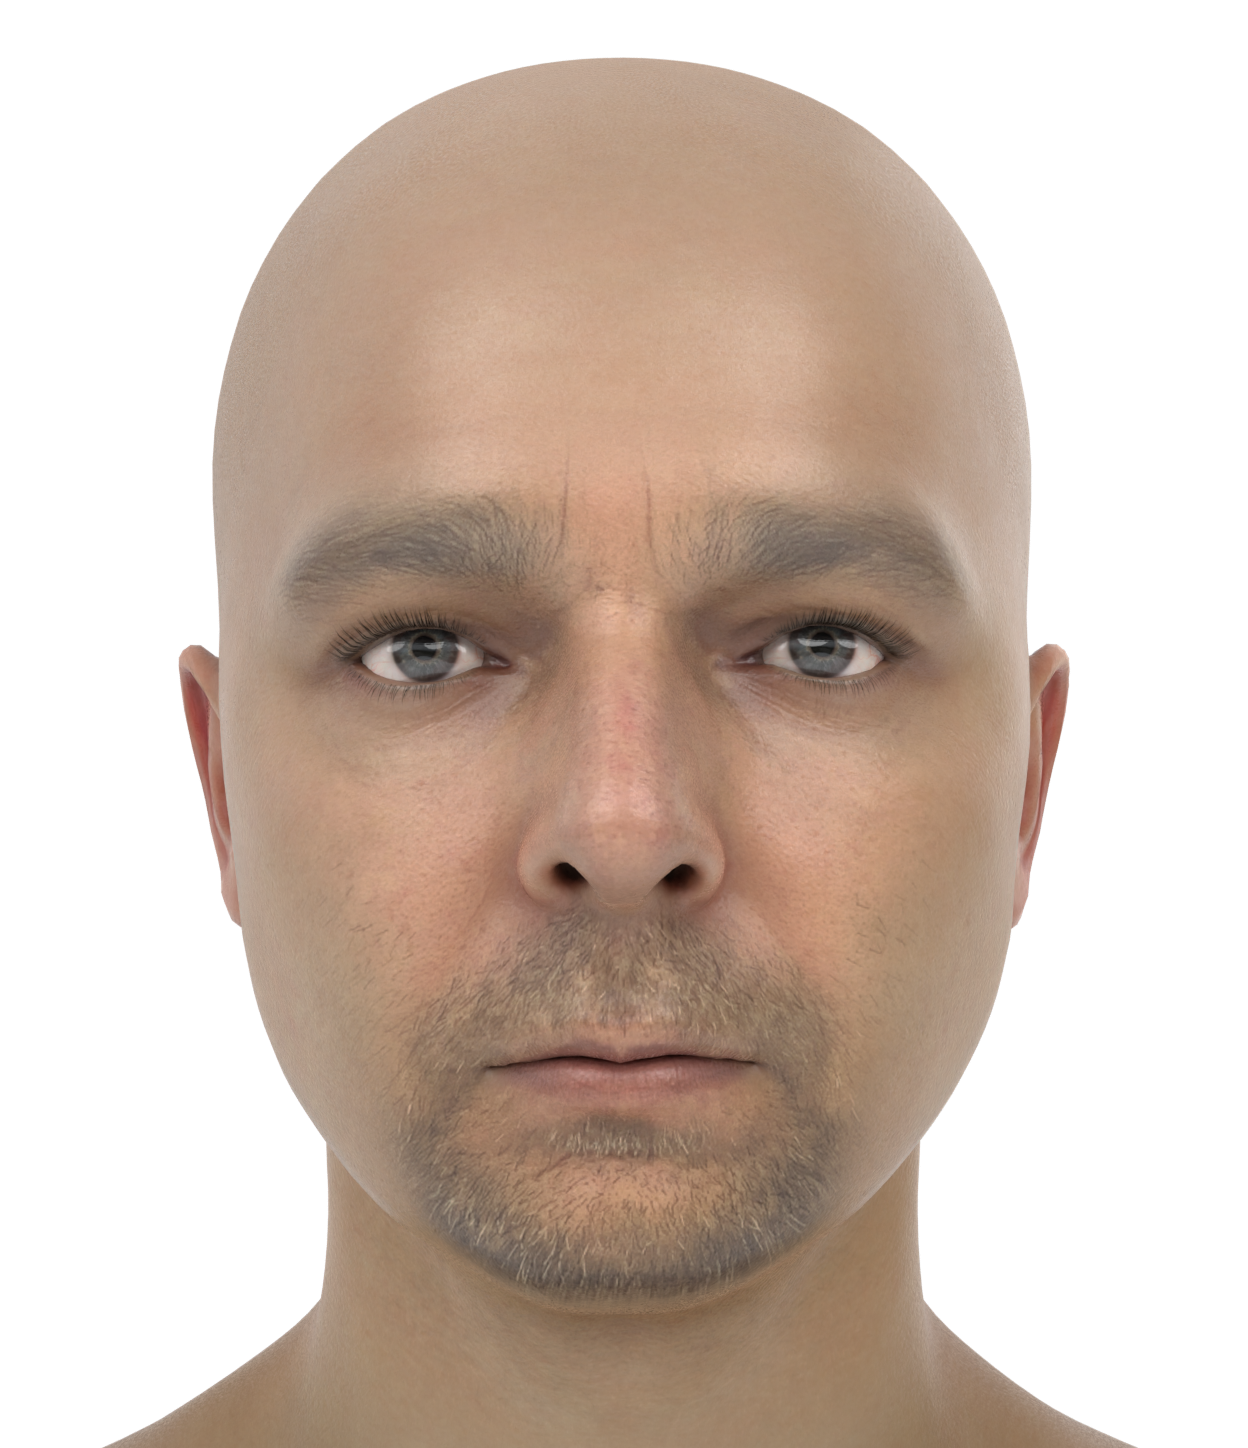
\includegraphics[width=0.65\textwidth]{alexis_didimo_cropped.png}\\
  {\scriptsize My (hairless) digital twin.}
\end{center}
\hfill\null

\vspace*{0.5ex} % Extra space after the picture

\headleft{Profile}
 Hands-on technical team leader, {\bf applied math} research engineer at heart, with a specialist expertise in {\bf computer vision} and {\bf computer graphics}. 

\headleft{Contact details}
\small % To fit more content
\MVAt\ {\small alexis.roche@gmail.com} \\[0.4ex]
\Mobilefone\ +351\,910\,327\,756 \\[0.5ex]
\Mundus\ \href{https://www.linkedin.com/in/alexis-roche-3815592}{LinkedIn profile} \\[0.1ex]
\Mundus\ \href{https://orcid.org/0000-0002-4821-6893}{ORCID profile} \\[0.1ex]
\Mundus\ \href{https://scholar.google.com/citations?user=LJJTi1gAAAAJ&hl}{Google Scholar profile} %\\[0.1ex]
%\Letter\ Porto, Portugal
\normalsize

\headleft{Personal information}
%\MALE \\[0.5ex]
%Year of birth: \textbf{1861} \\[0.5ex]
\Letter\ Porto, {\bf Portugal} \\[0.5ex]
Citizenship: {\bf France} \\[0.5ex]
%Family: \textbf{Single without children} \\[0.5ex]
Languages: {\bf English} (fluent), {\bf French} (native).

%\headleft{Skills}
%\begin{itemize}
%\item Python, SQL, PySpark
%\item R, Matlab, Azure Databricks
%\item MS Word, Excel, PowerPoint
%\item Communication and team collaboration
%\end{itemize} 

\end{minipage}%
\kern0.09\textwidth\relax%%Right margin provided explicitly to stretch the colourbox
}
\end{minipage}% Right column
\hskip2.5em% Left margin for the white area
\begin{minipage}[t]{0.56\textwidth}
\setlength{\parskip}{0.8ex}% Adds spaces between paragraphs; use \\ to add new lines without this space. Shrink this amount to fit more data vertically

\vspace{2ex}

\headright{Experience}

{\sc Head of Artificial Intelligence.} {\it Didimo}, Porto, Portugal. \hphantom{CACACACA} \dates{Sep 2019--present} \\
\smaller{Leading development of automated 3D character creation for {\em Popul8} software: shape reconstruction / generation, skin texturing, asset fitting, autorigging, autoskinning, mesh shrink-wrapping.}

\is % Item spacing -- defined in the preamble
{\sc Senior Computer Vision Scientist.} {\it CoVii (Ar\c celik/Beko R\& D center)}, Porto, Portugal. \dates{Feb 2017--Jul 2019} \\
\smaller{Developed embedded ML algorithms for smart domestic appliances: {\em VUXHub} and {\em Artisan oven} prototypes (demonstrated at IFA Berlin, 2017-18).}

\is
{\sc Lead Clinical Research.} {\it Siemens Healthineers / University Hospital (CHUV)}, Lausanne, Switzerland. \dates{Sep 2011--Jan 2017} \\
\smaller{Led development and validation of embedded brain morphometry for radiological reading (released in 2020 as {\em AI-Rad Companion Brain MR} solution).}

\is
{\sc Academic Guest.} {\it Federal Institute of Technology (ETHZ)}, Zurich, Switzerland. \dates{May 2009--Jul 2011} \\
\smaller{Advised the Computer Vision Lab (BIWI) on brain image analysis research.}

\is
{\sc Permanent Researcher.} {\it French Atomic Commission (CEA)}, Paris-Saclay, France. \dates{Dec 2002--Jul 2011} \\
\smaller{Investigated various brain MRI analysis methods at the Neurospin brain imaging center.}

\is
{\sc Post-doctoral research Assistant.} {\it University of Oxford}, United Kingdom. \dates{Apr 2001--Oct 2002} \\
\smaller{Developed medical image registration algorithms at the Wolfson Medical Vision Laboratory and consulted for Mirada Solutions Ltd.}

\headright{Education}

{\sc PhD in Engineering Science.} {\it INRIA / Universit\'e C\^ote d'Azur}, Sophia Antipolis, France. \dates{Sep 1997--Mar 2001}

\is
{\sc MsC in Cognitive Science.} {\it Sorbonne Universit\'e}, Paris, France. \hphantom{CACACACA} \dates{Sep 1995--Sep 1996}

\is
{\sc Centralien Engineer Degree (equivalent MsC).} {\it CentraleSup\'elec, Universit\'e Paris-Saclay}, France. \dates{Sep 1993--Jun 1996} 


\headright{Skills}

{\sc Technical leadership:} Proven ability to coordinate a technical team and manage objectives in multidisciplinary environments.

\is 
{\sc Collaborative programming:} Python (have used NumPy/SciPy since 2006), C, C++, Matlab, R, and using Git for version control.

\is 
{\sc Scientific writing:} Author of 106 peer-reviewed scientific articles and 6 published international patents. 8086 citations, {\em h}-index: 38.

\end{minipage}
\end{document}
